% Fig: end-to-end flow diagram (compiled separately with pdflatex)
\documentclass[border=2pt]{standalone}
\usepackage{mathptmx}
\usepackage{tikz}
\usetikzlibrary{arrows.meta,positioning,shapes.geometric,calc}
\begin{document}
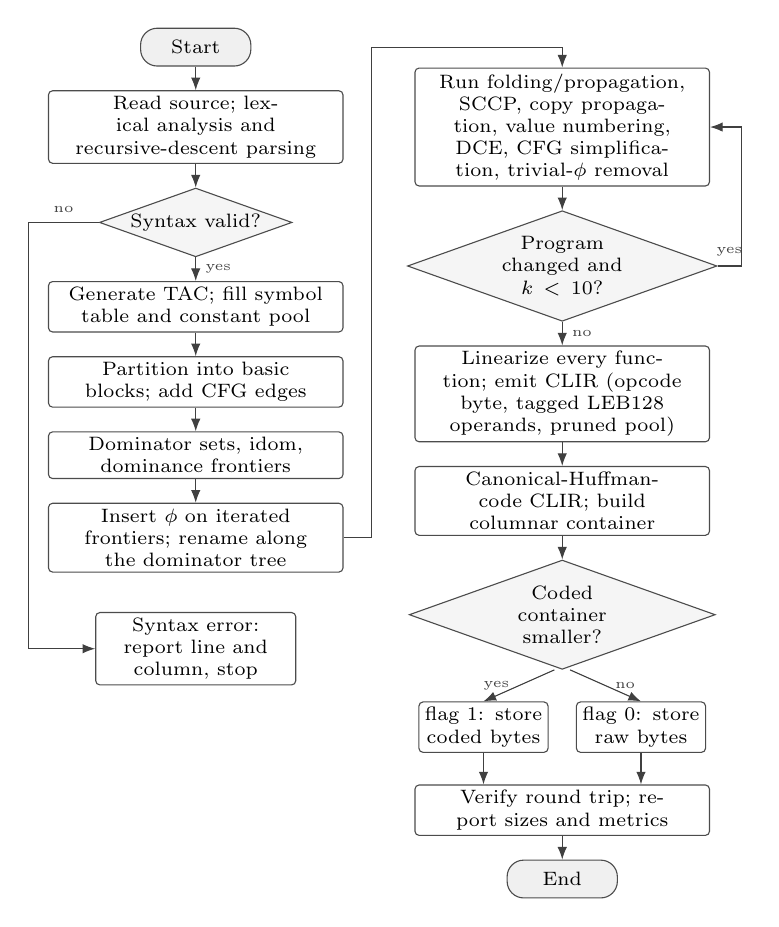
\begin{tikzpicture}[
  font=\scriptsize, node distance=3mm,
  proc/.style={draw=black!70, rounded corners=1.5pt, fill=white, align=center, text width=36mm, minimum height=5.5mm, inner sep=2pt},
  term/.style={draw=black!70, rounded corners=6pt, fill=black!6, align=center, minimum width=14mm, minimum height=4.8mm},
  dec/.style={draw=black!70, diamond, aspect=2.8, fill=black!4, align=center, inner sep=0.5pt, text width=17mm},
  arr/.style={-{Latex[length=1.6mm]}, black!75}]
  % ---------------- left column
  \node[term] (start) {Start};
  \node[proc, below=of start] (lex) {Read source; lexical analysis and recursive-descent parsing};
  \node[dec, below=of lex] (ok) {Syntax valid?};
  \node[proc, below=of ok] (tac) {Generate TAC; fill symbol table and constant pool};
  \node[proc, below=of tac] (cfg) {Partition into basic blocks; add CFG edges};
  \node[proc, below=of cfg] (dom) {Dominator sets, idom, dominance frontiers};
  \node[proc, below=of dom] (ssa) {Insert $\phi$ on iterated frontiers; rename along the dominator tree};
  \node[proc, below=5mm of ssa, text width=24mm] (err) {Syntax error: report line and column, stop};
  % ---------------- right column
  \node[proc, right=9mm of lex] (pass) {Run folding/propagation, SCCP, copy propagation, value numbering, DCE, CFG simplification, trivial-$\phi$ removal};
  \node[dec, below=of pass] (fix) {Program changed and $k<10$?};
  \node[proc, below=of fix] (clir) {Linearize every function; emit CLIR (opcode byte, tagged LEB128 operands, pruned pool)};
  \node[proc, below=of clir] (enc) {Canonical-Huffman-code CLIR; build columnar container};
  \node[dec, below=of enc] (small) {Coded container smaller?};
  \node[proc, below=4mm of small, xshift=-10mm, text width=15mm] (yes) {flag 1: store coded bytes};
  \node[proc, below=4mm of small, xshift=10mm, text width=15mm] (no) {flag 0: store raw bytes};
  \node[proc, below=4mm of $(yes.south)!0.5!(no.south)$] (rep) {Verify round trip; report sizes and metrics};
  \node[term, below=of rep] (end) {End};
  % ---------------- arrows
  \draw[arr] (start) -- (lex);
  \draw[arr] (lex) -- (ok);
  \draw[arr] (ok) -- node[right, font=\tiny]{yes} (tac);
  \draw[arr] (ok.west) -- node[above, font=\tiny]{no} ($(ok.west -| lex.west)+(-2.5mm,0)$) |- (err.west);
  \draw[arr] (tac) -- (cfg);
  \draw[arr] (cfg) -- (dom);
  \draw[arr] (dom) -- (ssa);
  \draw[arr] (ssa.east) -- ++(3.5mm,0) |- ($(pass.north)+(0,2.5mm)$) -- (pass.north);
  \draw[arr] (pass) -- (fix);
  \draw[arr] (fix.east) -- node[above, font=\tiny]{yes} ++(3mm,0) |- (pass.east);
  \draw[arr] (fix) -- node[right, font=\tiny]{no} (clir);
  \draw[arr] (clir) -- (enc);
  \draw[arr] (enc) -- (small);
  \draw[arr] (small.south) ++(-1mm,0) -- node[left, font=\tiny]{yes} (yes.north);
  \draw[arr] (small.south) ++(1mm,0) -- node[right, font=\tiny]{no} (no.north);
  \draw[arr] (yes.south) -- (rep.north -| yes.south);
  \draw[arr] (no.south) -- (rep.north -| no.south);
  \draw[arr] (rep) -- (end);
\end{tikzpicture}
\end{document}
